\section{Methodology}\label{sec3}

\subsection{Dynamic Graph Representation}
We represent the transportation system at snapshot time $t$ as a directed multi-relational graph
\begin{equation}
G_t = \big(V_t, E_t, \{A_t^{(\rho)}, W_t^{(\rho)}\}_{\rho\in\mathcal{R}}\big),
\end{equation}
where:
\begin{itemize}
    \item $V_t = V^j \cup V_t^v$ is the set of nodes at time $t$, consisting of
        \begin{itemize}
            \item $V^j$: static junction nodes, representing intersections in the road network,
            \item $V_t^v$: dynamic vehicle nodes, representing vehicles present at time $t$.
        \end{itemize}
    \item $E_t$ is the set of directed edges at time $t$, partitioned by relation type $\rho$.
    \item $\mathcal{R}$ is the set of relation types (road, traversal, interaction).
    \item $A_t^{(\rho)} \in \{0,1\}^{|V_t|\times |V_t|}$ is the binary adjacency matrix for relation $\rho$ at time $t$.
    \item $W_t^{(\rho)} \in \mathbb{R}_{\ge 0}^{|V_t|\times |V_t|}$ is the optional weighted adjacency for relation $\rho$ (e.g., distance-based interaction weights).
\end{itemize}

\begin{figure}[t]
    \centering
    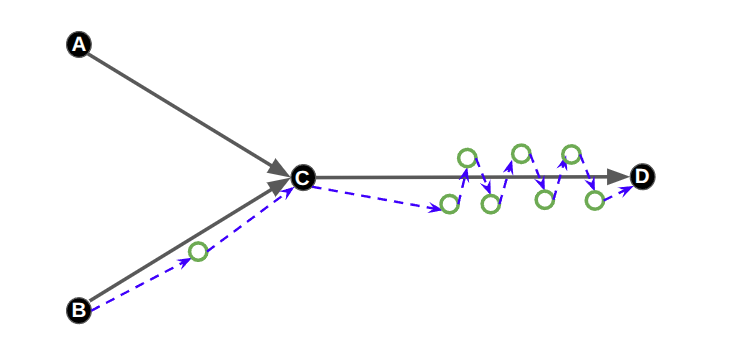
\includegraphics[width=0.8\linewidth]{figures/dynamic_nodes_edges.png}
    \caption{Dynamic, multi-relational traffic graph: static junction nodes (labeled A--D) and road edges (solid gray) with dynamic vehicle nodes (hollow green circles) and interaction edges (blue dashed).}\label{fig:dyn-graph}
\end{figure}

% Compact components figure: encoder, route encoder, router/MoE
\begin{figure}[t]
    \centering
    \subfloat[Graph encoder (last snapshot)]{\resizebox{0.85\columnwidth}{!}{\input{figures/fig_encoder.tikz}}}\\[2mm]
    \subfloat[Route encoder (vehicle intent)]{\resizebox{0.85\columnwidth}{!}{\input{figures/fig_route_encoder.tikz}}}\\[2mm]
    \subfloat[Router and Mixture-of-Experts]{\resizebox{0.85\columnwidth}{!}{\input{figures/fig_router_moe.tikz}}}
    \caption{Key components: (a) two-layer GATv2 with edge features; (b) route intent via edge-ID embeddings and mean pooling; (c) sparse Top-$k=2$ routing over six experts with load balancing.}\label{fig:components}
\end{figure}

We define three relation types:
\begin{enumerate}
    \item \textbf{Road edges ($\rho=\text{road}$):} For adjacent junctions $(u,v)$ with legal direction $u\!\to\!v$, we add $(u,v)\in E_t^{(\text{road})}$, encoding static road topology.
    \item \textbf{Traversal edges ($\rho=\text{trav}$):} If vehicle $v_i^t$ occupies segment $(a,b)$, we add $(a,v_i^t)$ and $(v_i^t,b)$, linking the vehicle to its upstream and downstream junctions.
    \item \textbf{Interaction edges ($\rho=\text{inter}$):} For vehicles $v_i^t,v_j^t$ on the same segment with spacing $d_{ij}(t)\le\varepsilon$ and aligned headings, we add $(v_i^t,v_j^t)$ weighted by $\omega(d_{ij}(t)) = e^{-d_{ij}(t)/\lambda}$.
\end{enumerate}

\paragraph{Dynamic edge construction.}
In implementation, vehicles on each road segment are ordered by their normalized position along the edge. We then create a short chain per segment: a junction$\to$first-vehicle edge (type 1), vehicle$\to$vehicle links along the ordered list (type 3), and last-vehicle$\to$junction (type 2). These dynamic edges sit on top of the static road graph (type 0).

Each node and edge carries feature vectors. Nodes use 28 features per snapshot (junction/vehicle type, kinematics, temporal encodings, zone one-hot, coordinates, current-edge attributes, demand/occupancy surrogates, and junction type). Edges use 7 features (average speed, lanes one-hot, length, demand, occupancy). Average speed, demand, and occupancy are updated per snapshot from data; vehicle features at indices for current-edge demand/occupancy are filled from the corresponding edge attributes.

\paragraph{Route intent.}
In addition to graph-based relations, each vehicle node includes a feature called \texttt{vehicle\_route\_left}, which encodes the sequence of upcoming edges along its pre-computed source--destination path. Construction: for each trip we compute a static shortest path over $E^{\mathrm{road}}$ and record its ordered edge-ID list. At time $t$, we locate the vehicle's current edge within this list and take the suffix from the next edge to the destination. Indices are the canonical 0-based edge IDs shared across the dataset (vocabulary size 1{,}294). This sequence is summarized by a Route Encoder (edge-ID embedding + mean pooling) and used in fusion.

\subsection{Temporal Windowing}
ETA prediction requires reasoning over temporal dynamics. We construct a window of $H$ consecutive snapshots:
\begin{equation}
\mathcal{G}_{t-H+1:t} = \{G_\tau\}_{\tau=t-H+1}^t,
\end{equation}
where $H$ is configurable (default $H{=}30$ in our experiments, with 30-second spacing). The prediction target is the ETA of vehicles present in the final snapshot $G_t$.

\subsection{Problem Statement}
Given a temporal window of dynamic graphs $\mathcal{G}_{t-H+1:t}=\{G_{\tau}\}_{\tau=t-H+1}^{t}$, where each snapshot $G_{\tau}$ contains static junction nodes $V^{j}$, dynamic vehicle nodes $V^{v}_{\tau}$, static road edges, and time-varying interaction edges, the goal is to predict per-vehicle ETAs at the final snapshot $t^*{=}t$. Let $\mathcal{V}_t = V^{v}_{t}$ denote vehicles present at time $t$. We learn a function $f_{\theta}$ that maps
\begin{equation}
f_{\theta}\big(\mathcal{G}_{t-H+1:t},\;\texttt{route\_left}\big) \;\to\; \hat{\mathbf{y}}_t \in \mathbb{R}^{|\mathcal{V}_t|},
\end{equation}
where $\hat{\mathbf{y}}_t[i]$ is the ETA for vehicle $i\in\mathcal{V}_t$. Training minimizes mean absolute error (MAE) over vehicles present at $t$ (additional terms are described in Section~\ref{sec:loss}):
\begin{equation}
\mathcal{L}_{\text{MAE}} = \frac{1}{|\mathcal{V}_t|}\sum_{i\in\mathcal{V}_t} \big| \hat{y}_t[i] - y_t[i] \big|.
\end{equation}

\subsection{Model Architecture}
Our DSTRA-GNN (Dynamic Spatio-Temporal Route-Aware GNN) integrates spatial, temporal, and route information. See the complete architecture in Fig.~\ref{fig:temporal-moe-eta}. The main components are:

\begin{itemize}
    \item \textbf{Graph Encoder:} Each snapshot $G_t$ is processed by a multi-layer GATv2-based encoder with residual connections and edge features, producing embeddings for junction and vehicle nodes (see the encoder panel in Fig.~\ref{fig:components}).
    \item \textbf{Temporal Aggregator:} For each pre-final snapshot $\tau\in\{t{-}H{+}1,\ldots,t{-}1\}$ we take the static road-edge features (edge\_type$=0$) and build edge-wise sequences across time. A temporal module (Transformer with sinusoidal positional encodings; GRU optional) processes these sequences per edge; the temporally aggregated edge features are then projected and pooled over all static edges to a graph-level context vector (detail in Fig.~\ref{fig:transformer-detail}). This context is broadcast to all vehicles at $t^*$ for prediction. For \emph{all} temporal variants, temporal context is computed from static road edges only for $t{-}H{+}1\ldots t{-}1$, while the final snapshot $G_t$ is encoded with the appropriate spatial topology (static or full dynamic) per variant.
    \item \textbf{Vehicle Selection:} From the final snapshot $G_t$, we retain only vehicle node embeddings, as these are the prediction targets for ETA.
    \item \textbf{Route Encoder:} Each vehicle's remaining route (\texttt{vehicle\_route\_left}) is embedded via an edge-ID lookup (vocabulary $|E^{\mathrm{road}}|{=}1{,}294$, embedding dim 64) followed by mean pooling over the variable-length sequence (see the route panel in Fig.~\ref{fig:components}). The pooled route vector is concatenated with the vehicle embedding and temporal context when route awareness is enabled.
    \item \textbf{Fusion and MoE Head:} Vehicle embeddings, enriched with route and temporal context, are fused through a feed-forward network and routed to a sparse Top-$k$ Mixture-of-Experts (MoE) head (router panel in Fig.~\ref{fig:components}), where specialized experts capture heterogeneous traffic regimes. The output is the ETA prediction for each vehicle.
\end{itemize}

% ===== TikZ Diagram of Model Architecture =====
\begin{figure*}[t]
    \centering
    \resizebox{0.88\textwidth}{!}{\input{figures/fig_temporal_moe_eta.tikz}}
    \caption{DSTRA-GNN architecture. A window of $T{=}30$ dynamic graph snapshots (shown as an overlapped deck) is processed by a \emph{shared} Graph Encoder; prediction is made at the last snapshot $t^*$. In the Full variant, a Route Encoder summarizes each vehicle's remaining path before Fusion and a Top-$k$ MoE head produces per-vehicle ETA.}\label{fig:temporal-moe-eta}
\end{figure*}

\begin{figure}[t]
    \centering
    \resizebox{\linewidth}{!}{\input{figures/fig_temporal_transformer_detail.tikz}}
    \caption{Temporal Transformer detail: per-edge sequences across $H{-}1$ snapshots are projected, positionally encoded, encoded by a Transformer stack, reduced via last-token + norm, projected back to edge dimension, then pooled over edges.}\label{fig:transformer-detail}
\end{figure}

\subsection{Model Configuration}
Unless stated otherwise, experiments use the following settings:
\begin{itemize}
    \item \textbf{Node/edge features}: 28 node features; 7 edge features. Temporal window $H{=}30$ consecutive snapshots.
    \item \textbf{Graph encoder}: 2-layer GATv2 with edge features, hidden size 128, 4 heads per layer, GELU activations, LayerNorm residuals, dropout 0.1.
    \item \textbf{Temporal module}: static-road edge sequences over the first $H{-}1$ snapshots. Default is a Transformer Encoder with $n_\text{head}{=}4$, $n_\text{layers}{=}2$, GELU, FFN size $2d$, dropout 0.1, and sinusoidal positional encodings; an optional single-layer GRU (hidden 128) is also supported. Aggregated edge context is projected, mean-pooled over static edges to a graph vector, then broadcast to vehicles.
    \item \textbf{Route encoder}: edge-ID embedding of size 64 with mean pooling over \texttt{vehicle\_route\_left} (vocabulary size 1294).
    \item \textbf{Fusion}: MLP  (256 hidden with GELU, LayerNorm, dropout 0.1) to a 192-dim fused representation.
    \item \textbf{MoE head}: Top-$k{=}2$ sparse routing over $6$ experts (dropout 0.1). Predictions are made for vehicles in the last snapshot only.
    \item \textbf{Target normalization}: we train in the $y_{log,z}$ space:
    \begin{equation}
    y_{log} = \log\big(1 + y_{sec}\big)
    \end{equation}
    \begin{equation}
    y_{log,z} = \frac{y_{log} - \mu}{\sigma}
    \end{equation}
    where $y_{sec}$ is the raw ETA in seconds, and $(\mu,\sigma)$ are computed on the training set; metrics are reported after inverting to seconds.
    \item \textbf{Training}: AdamW (lr $10^{-3}$, weight decay $10^{-2}$), linear warmup then cosine annealing ($T_{\text{max}}{=}200$), batch size 2, 200 epochs. Primary loss in target space with metrics reported after inversion to seconds.
    \item \textbf{Router regularization}: load-balancing weight $\lambda_\text{lb}{=}0.05$ plus optional KL-to-uniform router regularization with weight 0.002.
\end{itemize}

\subsection{Loss Functions and Training Protocol}\label{sec:loss}
We train the model with supervised regression on ETA targets using mean absolute error (MAE) in seconds:
\begin{equation}
\mathcal{L}_{\text{MAE}} = \frac{1}{N}\sum_{i=1}^N \big| \hat{y}_i - y_i \big|,
\end{equation}
where $\hat{y}_i$ and $y_i$ are the predicted and true ETAs. Additional evaluation metrics include RMSE and mean absolute percentage error (MAPE). The optimization objective includes MoE load balancing and optional router regularization:
\begin{equation}
\mathcal{L} = \mathcal{L}_{\text{reg}} + \lambda_{\text{lb}}\,\mathcal{L}_{\text{lb}} \;\; (\text{and optionally } 
\lambda_{\text{kl}}\,\mathrm{KL}(p\,\Vert\,\text{Uniform})),
\end{equation}
where $\mathcal{L}_{\text{lb}}$ encourages uniform expert usage via importance/load terms from the router, and $p$ are routing probabilities. Training occurs in a chosen target space (e.g., $y_{\text{log}}$ or $y_{\text{log\_z}}$), while metrics are reported after consistent inversion to seconds.

For completeness, we report the following definitions used in evaluation:
\begin{equation}
\mathrm{RMSE} = \sqrt{\frac{1}{N}\sum_{i=1}^{N} (\hat{y}_i - y_i)^2}
\end{equation}
\begin{equation}
\mathrm{MAPE}(\%) = 100\cdot \frac{1}{N}\sum_{i=1}^{N} \left|\frac{\hat{y}_i - y_i}{y_i}\right|
\end{equation}
All metrics are computed in seconds (after inverting any target-space transforms) and averaged over vehicles in the test split.

\paragraph{Complexity and inference.}
Per-snapshot spatial encoding is $\mathcal{O}(|E_t|)$; temporal aggregation is $\mathcal{O}(|E_\text{road}|\cdot(H{-}1))$ over static road edges only. Inference processes a window and emits per-vehicle ETAs at $t^*$ with negligible overhead beyond a single forward pass of the encoder plus temporal aggregator.

